\documentclass{article}
\usepackage[utf8]{inputenc}
\usepackage[english]{babel}
\usepackage[margin=2.5cm]{geometry}
\usepackage{graphicx}
\usepackage{amsmath}
\newtheorem{exercise}{\Large Zadatak}
\usepackage[export]{adjustbox}
\usepackage{caption}
\usepackage{subcaption}
\usepackage{fancyhdr}

\usepackage{listings}
\usepackage{xcolor}
% Kod
\definecolor{codegreen}{rgb}{0,0.6,0}
\definecolor{codegray}{rgb}{0.5,0.5,0.5}
\definecolor{codepurple}{rgb}{0.58,0,0.82}
\definecolor{backcolour}{rgb}{0.95,0.95,0.92}

\lstdefinestyle{mystyle}{
    backgroundcolor=\color{backcolour},   
    commentstyle=\color{codegreen},
    keywordstyle=\color{magenta},
    numberstyle=\tiny\color{codegray},
    stringstyle=\color{codepurple},
    basicstyle=\ttfamily\footnotesize,
    breakatwhitespace=false,         
    breaklines=true,                 
    captionpos=b,                    
    keepspaces=true,                 
    numbers=left,                    
    numbersep=5pt,                  
    showspaces=false,                
    showstringspaces=false,
    showtabs=false,                  
    tabsize=2
}

\lstset{style=mystyle}
\pagestyle{fancy}
\fancyhf{}



\lhead{13E053DOS - Domaći zadatak}
\rhead{Mladen Bašić 2018/0111} % Promeniti ime i dodati broj indeksa
% U fajlu design/intro.tex promeniti ime i prezime, broj indeksa i uneti parametre, a zatim u svakom zadatku iz foldera exercises uneti rešenja na odgovarajućim mestima. 

\begin{document}


\thispagestyle{empty}
	
	\begin{figure}[ht]
	   \minipage{0.15\textwidth}
			
\includegraphics[width=2.9cm]{design/logo_ETF.png}
	   \endminipage
	   \minipage{0.7\textwidth}
	   \begin{center}
	       \Large Univerzitet u Beogradu - Elektrotehnički fakultet \\ \Large Katedra za Signale i sisteme 
	   \end{center}
			
	   \endminipage
	   \minipage{0.16\textwidth}
			
\includegraphics[height = 3.2cm ,width=3.2cm]{design/logo_SIS.png}
		\endminipage
	\end{figure}
	
	\begin{center}
	\vspace{3.4cm}
	\LARGE
	13E053DOS - Digitalna obrada signala
	
	\vspace{0.8cm}
	\LARGE
	Domaći zadatak 
	
	
	\vspace{3cm}
	\normalsize	
	STUDENT \\
	\vspace{.3cm}
	\large
	\textbf{Mladen Bašić}
	
	\vspace{1.3cm}
	\normalsize	
	BROJ INDEKSA \\
	\vspace{.3cm}
	\large
	\textbf{2018/0111}
	
	\vspace{1.3cm}
	\normalsize	
	PARAMETRI \\
	\vspace{.3cm}
	\large
    \begin{tabular}{c c c c}
         P = 3& Q = 3& R = 1& S = 1 \\
    \end{tabular}	
	
    \vspace{3.5cm}
	\large
	\textbf{Decembar 2020.}
	\end{center}
	
	\newpage

\begin{exercise}
    
\begin{itemize}
    \item Parametar P = 3
    \item Analitički oblik signala $x[n]$ i $y[n]$ i broj tačaka $N$
    \begin{align*}
        x[n] &= \begin{cases} 
        n & 0 \leq n \leq 19 \\
        n - 19 & inace
        \end{cases} \\
        y[n] &= \begin{cases}
            2\cos(4n + \frac{\pi}{4}) & 0 \leq n \leq 19 \\
            0 & inace
        \end{cases}\\
        N &= 40
    \end{align*}
    \item Prikaz signala $x[n]$ i $y[n]$
    
        \begin{center}
            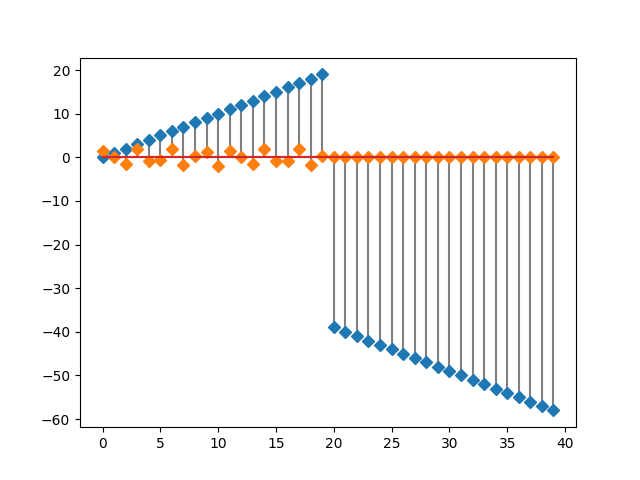
\includegraphics[width=0.7\textwidth]{figures/zad1_signali.png}
        \end{center}
    
    \item Prikaz rezultata linearne konvolucije i rezulata funkcije \textit{conv}
    	
        \begin{center}
            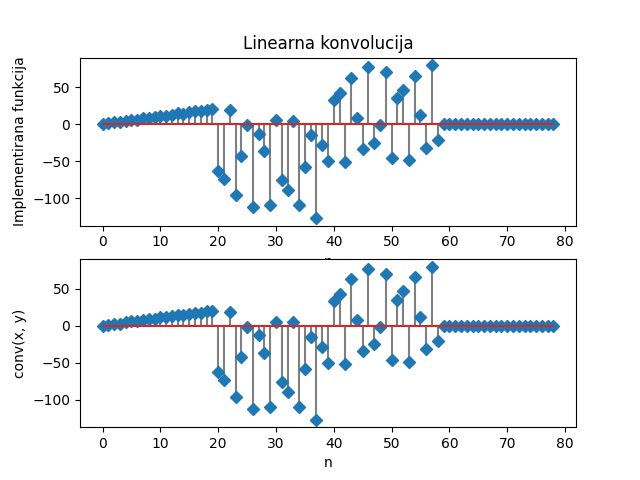
\includegraphics[width=0.7\textwidth]{figures/zad1_linearna_konvolucija.png}
        \end{center}
        
    \item Prikaz rezultata ciklične konvolucije i rezulata funkcije \textit{cconv}
    
        \begin{center}
            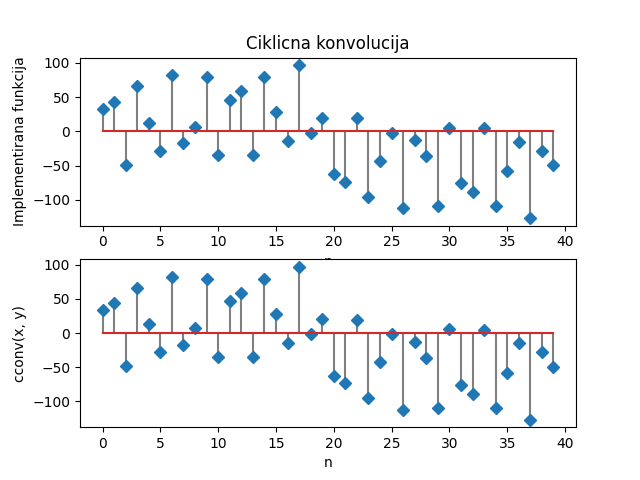
\includegraphics[width=0.7\textwidth]{figures/zad1_ciklicna_konvolucija_provera.png}
        \end{center}
        

    \item Linearna i ciklična konvolucija imaju iste vrednosti u sledećim odbircima
    
        \begin{center}
            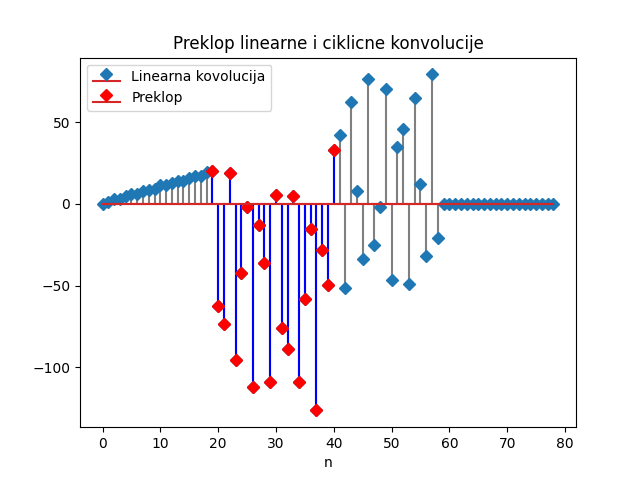
\includegraphics[width=0.7\textwidth]{figures/zad1_overlap.png}
        \end{center}
    
    \item{Programski k\^{o}d}
    \lstinputlisting[language=Python]{code/zad1.py}
  
\end{itemize}


\end{exercise}

\newpage
\begin{exercise}
    
\begin{itemize}
    \item Parametar Q = 
    \item Prikaz originalnog signala i signala dobijenog odabiranjem sa $f_S$ iz tabele
    \item Amplitudska frekvencijska karakteristika originalnog signala
    \item Signal se sastoji od sledećih tonova
    \item Programski k\^{o}d 
\end{itemize}


\end{exercise}

\newpage
\begin{exercise}
    
\begin{itemize}
    \item Parametar R = 1
    \item EKG signal u vremenskom domenu
        \begin{center}
            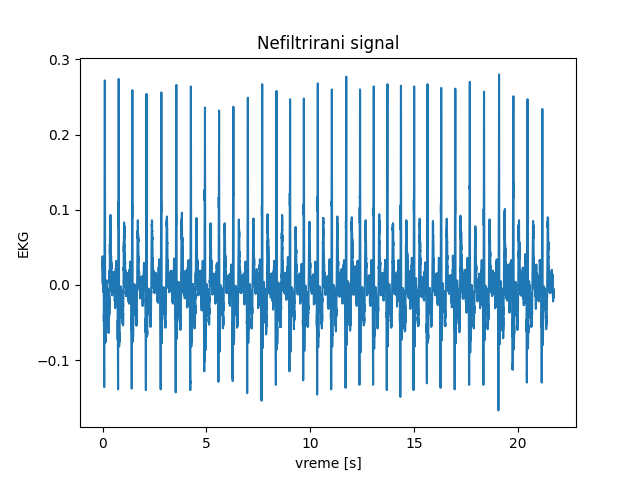
\includegraphics[width=0.7\textwidth]{figures/zad3_signal_vreme.png}
        \end{center}
        
    \item Amplitudska frekvencijska karakteristika EKG signala
        \begin{center}
            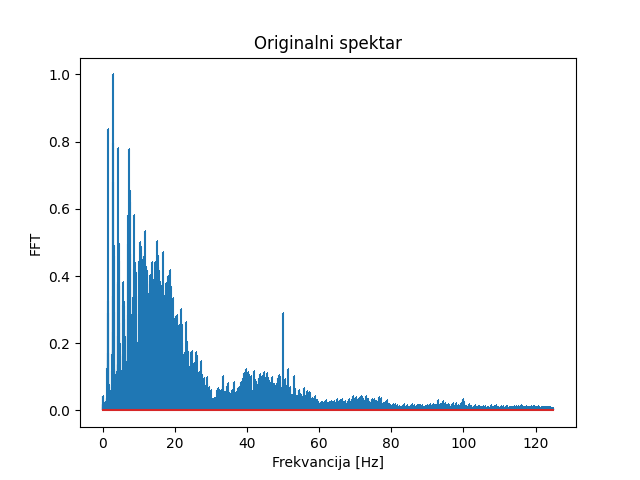
\includegraphics[width=0.7\textwidth]{figures/zad3_signal_spektar.png}
        \end{center}
        
    \item Amplitudske frekvencijske karakteristika analognih i digitalnih filtara
        \begin{center}
            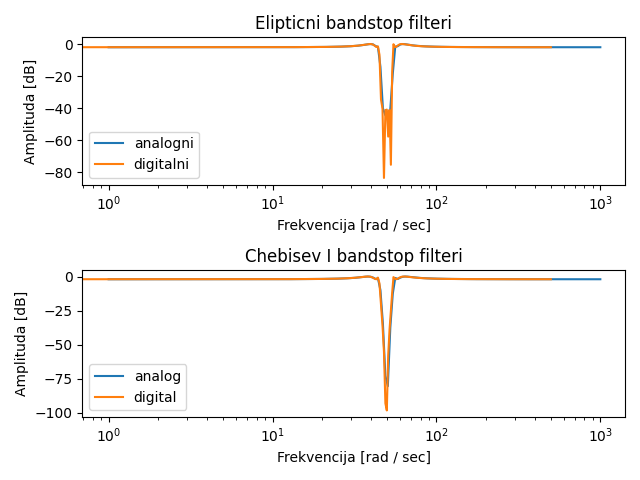
\includegraphics[width=0.7\textwidth]{figures/zad3_filteri.png}
        \end{center}
        
    \item Originalni i filtrirani signali u vremenskom domenu
        \begin{center}
            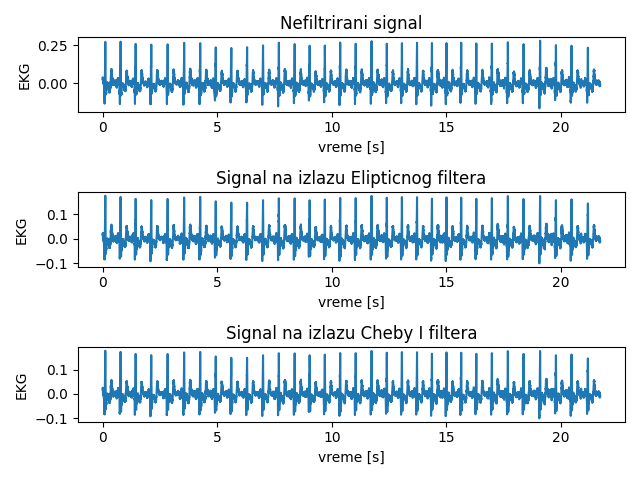
\includegraphics[width=0.7\textwidth]{figures/zad3_filtrirani_vreme.png}
        \end{center}
        
    \item Amplitudske frekvencijske karakteristika originalnog i filtriranih signala
        \begin{center}
            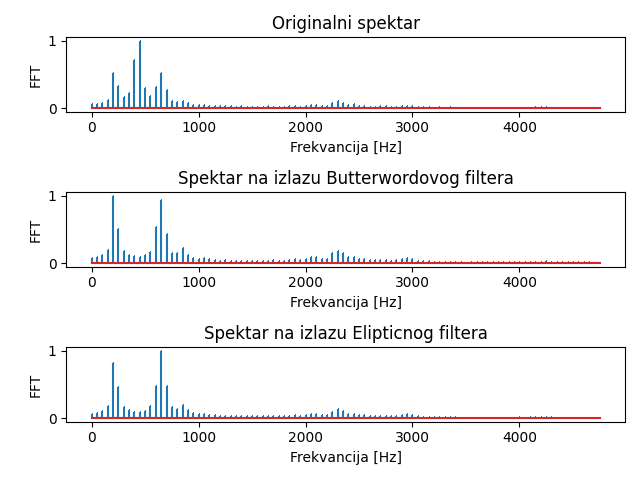
\includegraphics[width=0.7\textwidth]{figures/zad3_filtrirani_spektar.png}
        \end{center}
        
    \item Programski k\^{o}d 
    \lstinputlisting[language=Python]{code/zad3.py}
\end{itemize}
\end{exercise}

\newpage
\begin{exercise}
    
\begin{itemize}
    \item Parametar S = 1
    \item Snimak samoglasnika u vremenskom domenu
        \begin{center}
            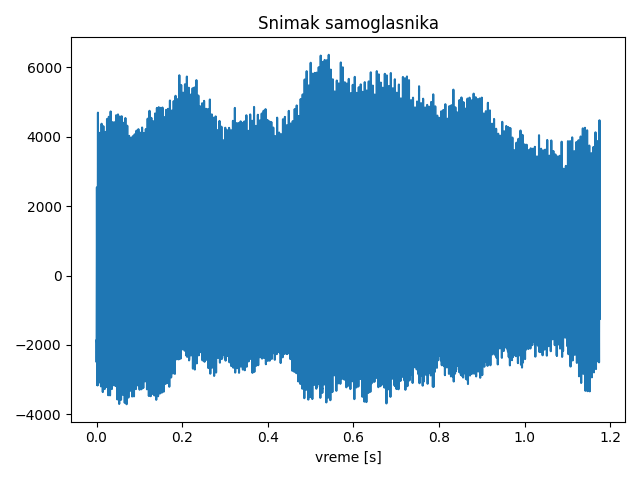
\includegraphics[width=0.7\textwidth]{figures/zad4_signal_vreme.png}
        \end{center}
        
    \item Usrednjena amplitudska frekvencijska karakteristika snimljenog signala
        \begin{center}
            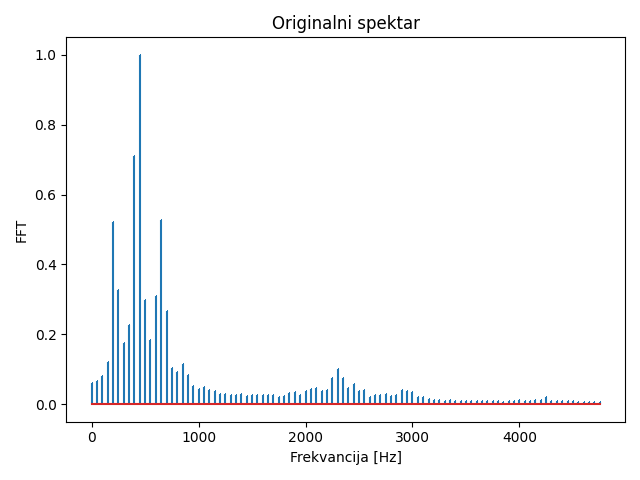
\includegraphics[width=0.7\textwidth]{figures/zad4_signal_spektar.png}
        \end{center}
        
    \item Amplitudske frekvencijske karakteristike projektovanih filtara
        \begin{center}
            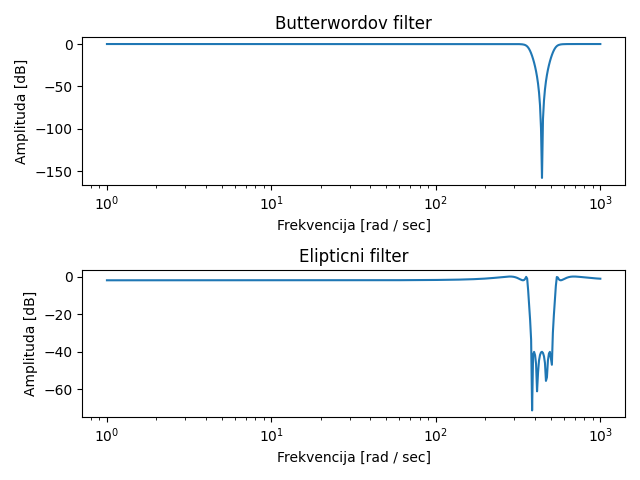
\includegraphics[width=0.7\textwidth]{figures/zad4_filteri.png}
        \end{center}
        
    \item Originalni i filtrirani signali u vremenskom domenu
        \begin{center}
            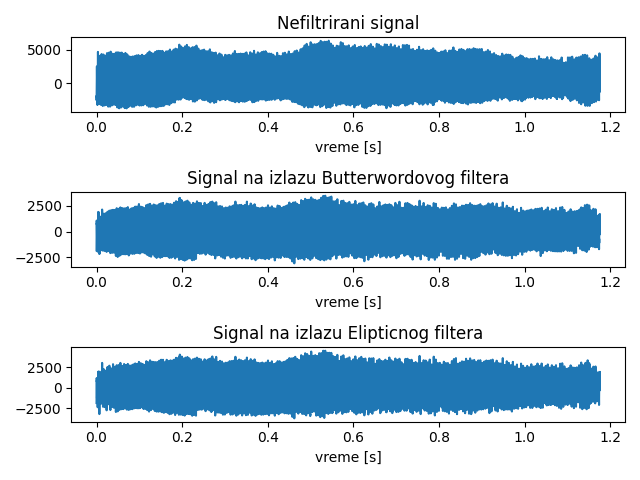
\includegraphics[width=0.7\textwidth]{figures/zad4_filtrirani_vreme.png}
        \end{center}
        
     \item Amplitudske frekvencijske karakteristike originalnog i filtriranih signala
         \begin{center}
            \includegraphics[width=0.7\textwidth]{figures/zad4_filtrirani_spektar.png}
        \end{center}
    \item Programski k\^{o}d 
    \lstinputlisting[language=Python]{code/zad3.py}
    
    \item Bonus - k\^{o}d i rezultati
    \lstinputlisting[language=Python]{code/bonus.py}
    Pitch frekvencija je 200Hz
\end{itemize}
\end{exercise}

\end{document}